% !TEX root = MusicFormatsCLIUserGuide.tex

\documentclass{beamer}

\mode<article>
{
  \usepackage{fullpage}
  \usepackage{pgf}
  \usepackage{hyperref}
  \setjobnamebeamerversion{vemus-smc07}
}

\mode<presentation>
{
  \usetheme{Frankfurt}
  \setbeamercovered{transparent}
  % or whatever (possibly just delete it)
}

\usepackage[english]{babel}
\usepackage[latin1]{inputenc}
\usepackage{times}
\usepackage[T1]{fontenc}
\usepackage{listings}
% Or whatever. Note that the encoding and the font should match. If T1
% does not look nice, try deleting the line with the fontenc.


\newcommand{\lcolorb}[1]{\color<#1>[rgb]{0,0,1}}
%\includeonlyframes{current}

\title % (optional, use only with long paper titles)
{MusicXML Library Version 2}{

\subtitle
{A toolbox to support the MusicXML format.}

\author[D.Fober] % (optional, use only with lots of authors)
{D.Fober, S.Letz, Y.Orlarey\\
{\scriptsize \{fober, letz, orlarey\}@grame.fr}}

\institute[Grame] % (optional, but mostly needed)
{
Grame - Research Lab.\\
Centre national de création musicale\\
FR - Lyon
}

\date[May 2008]
{May 2008}


\begin{document}

\begin{frame}
  \titlepage
\end{frame}


\begin{frame}{Summary}
  \tableofcontents
\end{frame}


%________________________________________________________________________
\chapter{Introduction}
%________________________________________________________________________
\section{The MusicXML format}
\begin{frame}
  \frametitle{The MusicXML format}
  The MusicXML format represents common Western musical notation from the 17th century onwards.
  It is an xml format that organizes the music into a header followed by the core
  music data.  The core music data may be organized as \emph{partwise} or \emph{timewise} data:
  
\begin{itemize}
    \item \emph{partwise} data are organized into parts containing measures,
    \item \emph{timewise} data are organized into measures containing parts.
  \end{itemize}
  The music notation complexity is reflected by the significant number of MusicXML elements:
  \alert{343} elements are defined by the version 2.0 of the format.
  \begin{block}{}
    {\small More details and DTDs on} \texttt{http://www.recordare.com/}
  \end{block}
\end{frame}


%________________________________________________________________________
\section{Issues in the library design}
\begin{frame}
  \frametitle{Issues in the library design}
  The main issues in designing a C++ library to support the format are related to the significant
  the number of MusicXML elements.
  \begin{enumerate}
    \item cost of describing all the MusicXML element,
    \item design of an adequate and efficient memory representation,
    \item avoiding additional complexity to the MusicXML format,
    \item easiness to maintain and to update to new versions of the format.
  \end{enumerate}

  \begin{block}{}
  The first version of the MusicXML library was quite good on points 2 and 3, but rather weak
  on points 1 and 4.
  \end{block}
\end{frame}


%________________________________________________________________________
\chapter{Overview}
%________________________________________________________________________
\section{Differences to version 1}
\begin{frame}
  \frametitle{libmusicxml v.2: what's new?}
  
\begin{itemize}
    \item supports the MusicXML format version 2,
    \item easy to upgrade to new versions of the MusicXML format from the DTDs,
    \item adheres strictly to the MusicXML DTDs: each element has a corresponding C++ class,
    \item designed using a single homogeneous \texttt{xmlelement} class and automatic
    typing using templates,
    \item provides STL iterators to browse the memory representation,
    \item is \alert{not compatible} with libmusicxml version 1.xx,
  \end{itemize}
  \begin{block}{}
  The main point is the simplified design: 4 classes instead of 150 to build a MusicXML
  memory representation.
  \end{block}
\end{frame}

%________________________________________________________________________
\section{What remains unchanged?}
\begin{frame}
  \frametitle{libmusicxml v.2: what remains unchanged?}
  
\begin{itemize}
    \item automatic memory management using smart pointers,
    \item support of the \texttt{visitor} mechanism,
    \item provides rolled and unrolled browsing,
    \item provides previous visitors (musicxml2guido, midivisitor, transposition...)
  \end{itemize}
\end{frame}


%________________________________________________________________________
\chapter{Inside the new library}
%________________________________________________________________________
\section{Class design}
\begin{frame}
  \frametitle{Memory representation}
  \begin{columns}
    \begin{column}[c]{7cm}
    The MusicXML format is represented by:
    {\small
        
\begin{itemize}
        \item<1-> a single \texttt{xmlelement} class
        \item<3-> simple methods to query an element
        \item<5-> derived into as many types as MusicXML elements using templates
        \item<7-> organized into a tree
        \end{itemize}}
    \end{column}

    \begin{column}[c]{5cm}
    \begin{overlayarea}{\textwidth}{50mm}
    {\small
      \only<1>{\vspace{8mm} 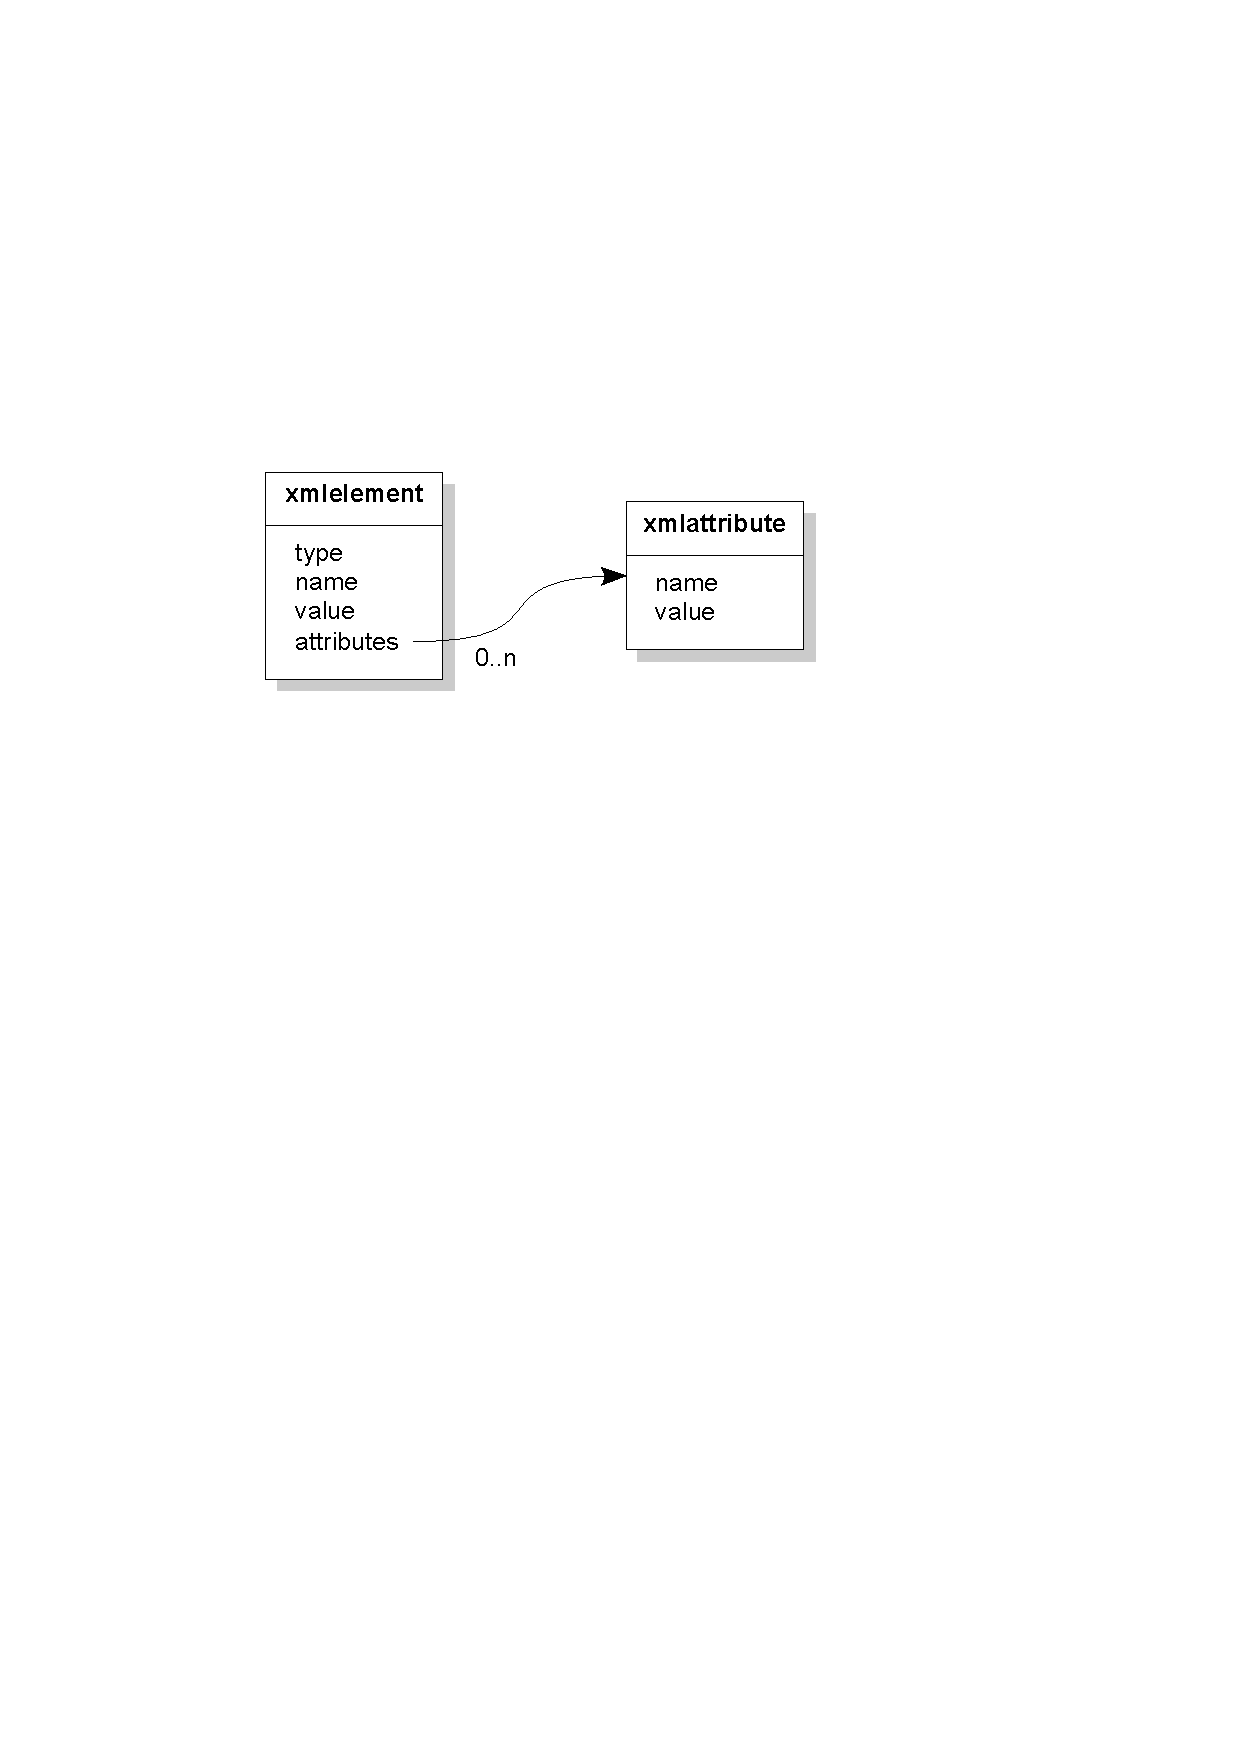
\includegraphics[width=50mm]{imgs/xmlelement.pdf}}
      \only<2>{\vspace{8mm} \begin{block}{}
      homogeneous design leads to simplicity.
        \end{block}}
      \only<3> {\vspace{9mm} 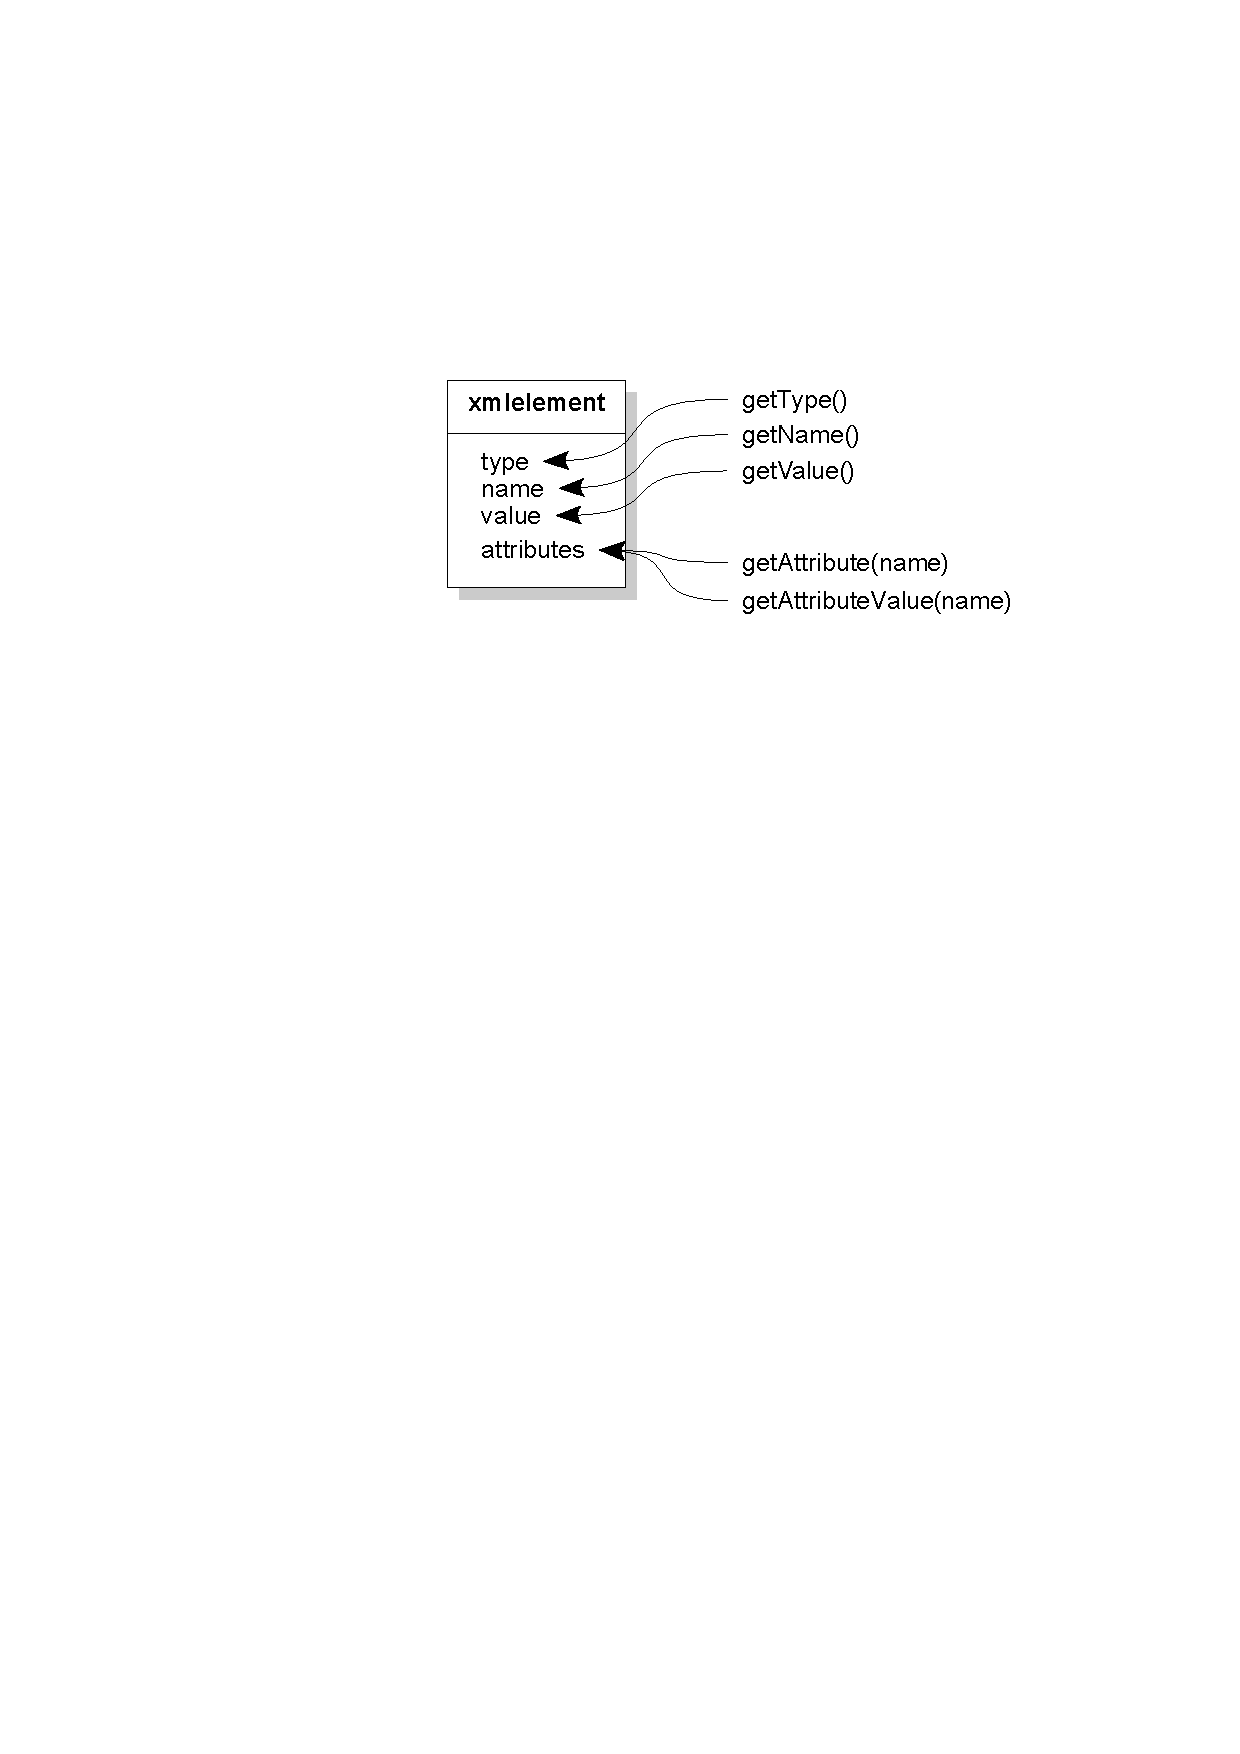
\includegraphics[width=50mm]{imgs/methods.pdf}}
     \only<4> {\vspace{9mm} \begin{block}{}
        Makes the DTDs usable as the library documentation:\\
        e.g. {\tiny \texttt{measure->getAttributeValue("number")}}
        \end{block}}
       \only<5> {\vspace{12mm}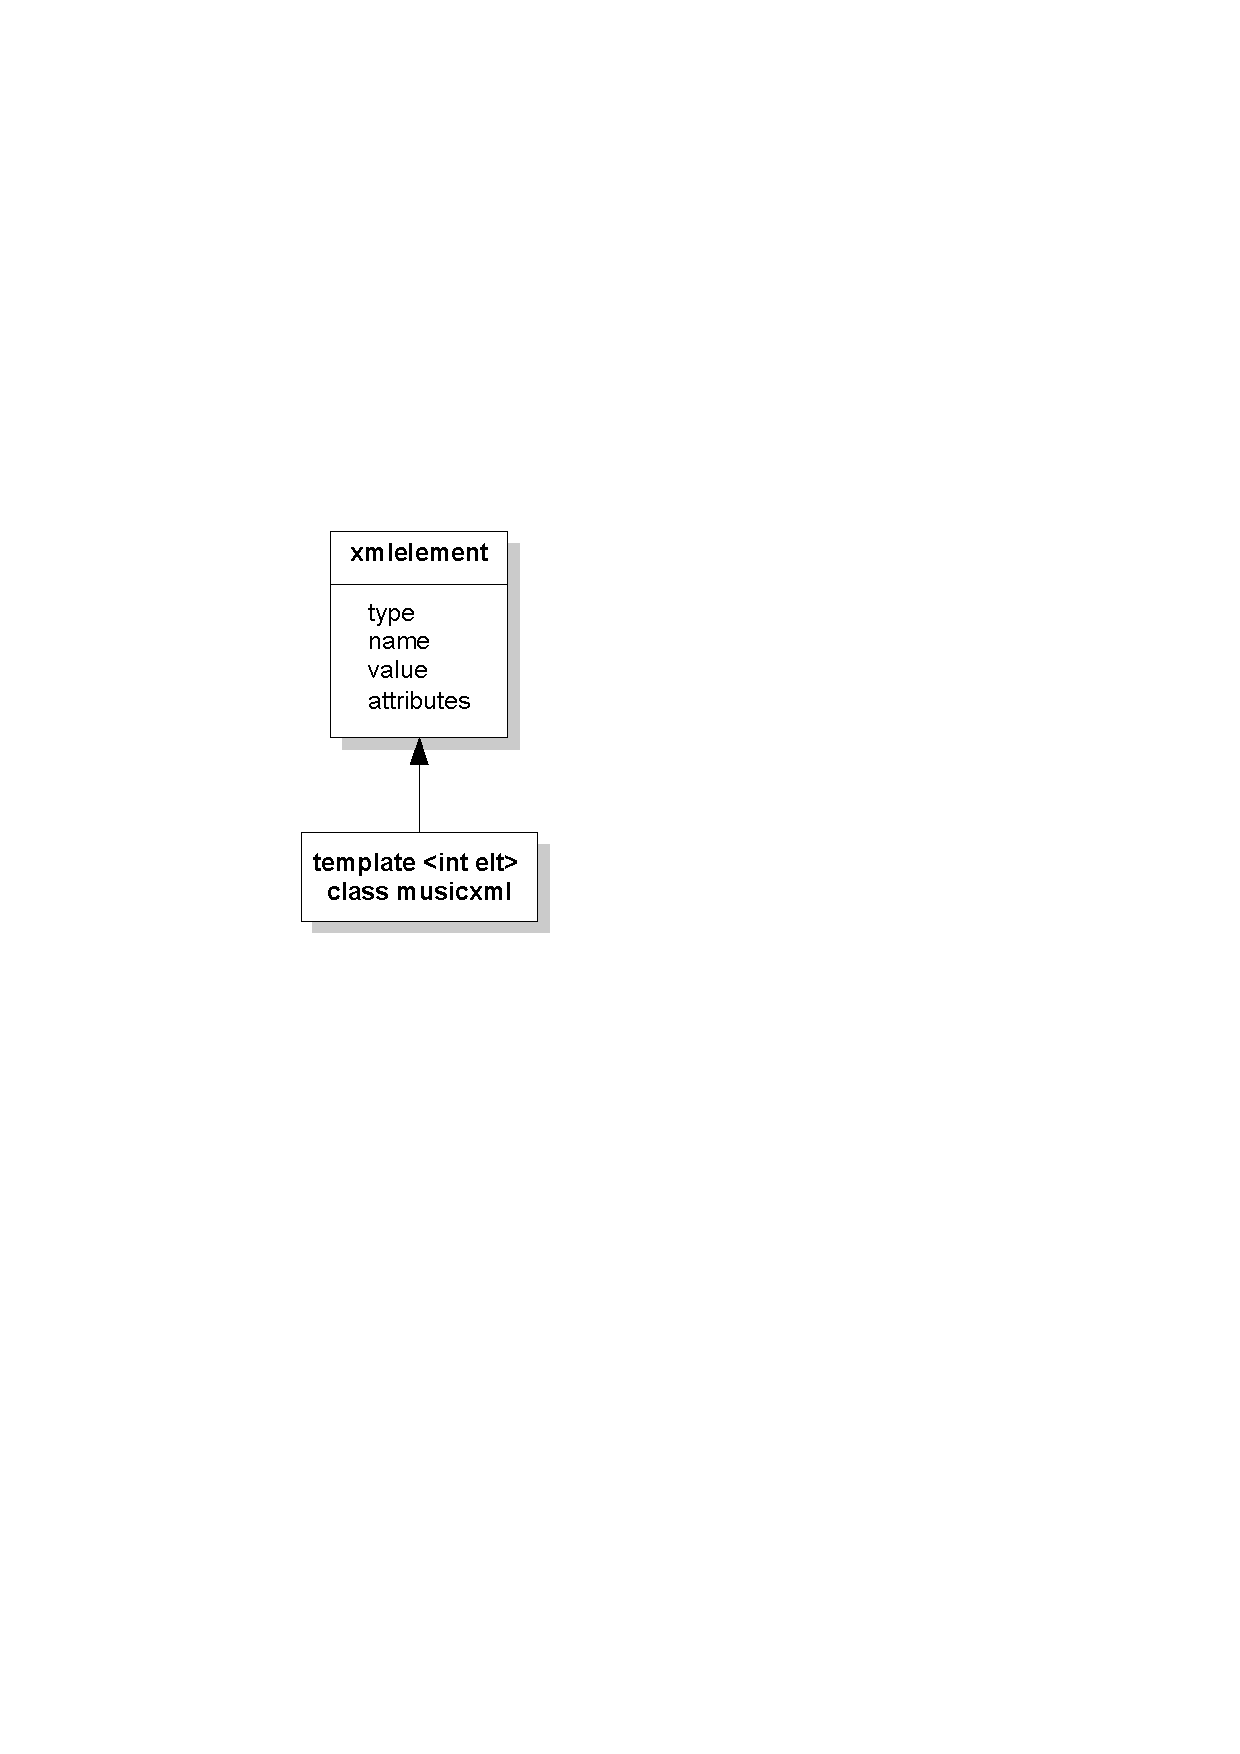
\includegraphics[width=25mm]{imgs/musicxml.pdf}}
     \only<6> {\vspace{22mm} \begin{block}{}
        Allows the visitor mechanism to operate
        \end{block}}
      \only<7> {\vspace{12mm} 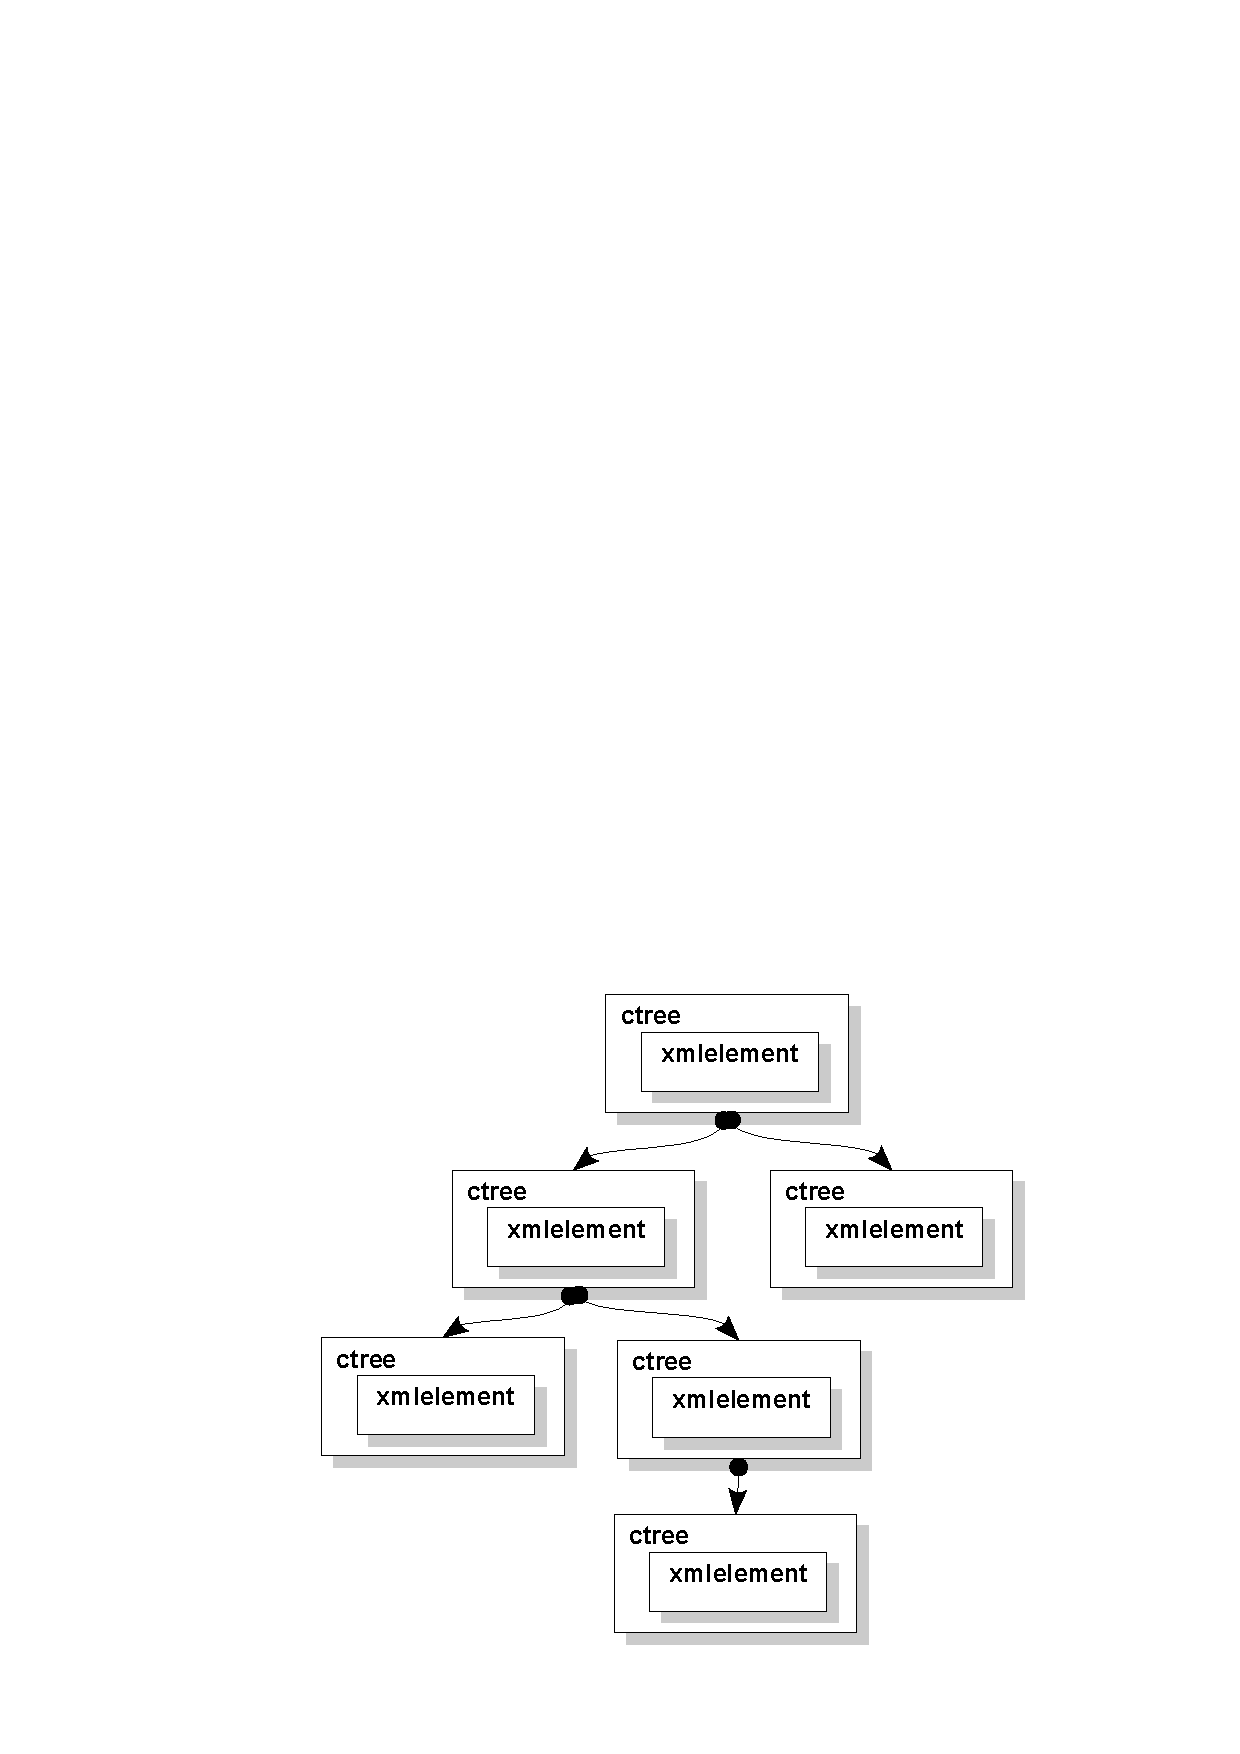
\includegraphics[width=50mm]{imgs/ctree.pdf}}
      \only<8> {\vspace{32mm} \begin{block}{}
        support STL iterators
        \end{block}}
    }
    \end{overlayarea}
    \end{column}
  \end{columns}
\end{frame}

%________________________________________________________________________
\section{DTDs as Documentation}
\begin{frame}
  \frametitle{MusicXML DTDs as documentation}
  \begin{columns}
    \begin{column}[c]{55mm}
    
\begin{itemize}
      \item<1-> types are consistently derived from the MusicXML element names
      \item<2-> attributes can be retrieved using their MusicXML names
      \item<3-> browsing the memory representation is like reading the MusicXML file
     \end{itemize}
    \end{column}
    \begin{column}[c]{60mm}
      \onslide<1->{
      \begin{block}{}
      {\scriptsize <!ELEMENT \alert{part-name}> \\
        \hspace{2mm} => class: \hspace{3mm} \alert{S\_part\_name} \\
        \hspace{2mm} => constant: \alert{k\_part\_name} }
      \end{block}}
      \onslide<2->{
      \begin{block}{}
      {\scriptsize <!ATTLIST \alert{measure} \\
      \hspace{13mm} \alert{number} CDATA \#REQUIRED \\
      \hspace{13mm} ...} \\
       {\tiny \texttt{measure->\alert{getAttributeValue("number")}
      measure->\alert{getAttributeIntValue("number",default)}}}
      \end{block}}
      \onslide<3->{
      \begin{block}{}
      {\scriptsize
      
\begin{itemize}
        \item Element and attributes names and values are available as string
          but support also automatic conversion to numeric types.
        \item Supports xml comments and processing instruction as well.
        \end{itemize}
      }
      \end{block}}
    \end{column}
  \end{columns}
\end{frame}

%________________________________________________________________________
\section{Browsing the memory representation}
\begin{frame}[fragile]
  \frametitle{Browsing the memory representation}
   \lstset{language=CPlusPlus, basicstyle=\tiny, emph={countnotes}, emphstyle=\color{red}}

  \begin{columns}
    \begin{column}[c]{50mm}
    
\begin{itemize}
      \item<1-> supports the acyclic visitor pattern
    \vspace{25mm}
      \item<2-> supports STL iterators
     \end{itemize}
    \end{column}

    \begin{column}[c]{65mm}
    \begin{block}<1->{Count using a visitor}
\begin{lstlisting}
class countnotes : public visitor<S_note>
{
    public:
    int fCount;

             countnotes() : fCount(0) {}
    virtual ~countnotes() {}
    void visitStart( S_note& elt ) { fCount++; }
};
\end{lstlisting}
    \end{block}

    \begin{block}<2->{Count using iterators and STL}
\begin{lstlisting}
struct countnotes {
    Bool operator () (const Sxmlelement elt) const
         return elt->getType() == k_note;
};

countnotes p;
int count = count_if(elt->begin(), elt->end(), p);
\end{lstlisting}
    \end{block}
    \end{column}
  \end{columns}
\end{frame}

%________________________________________________________________________
\section{Main files}
\begin{frame}
  \frametitle{Main files}

  {\small
  \begin{center}
  \begin{tabular}{|r|l|}
  \hline
  \textbf{Files, folders} & \textbf{Purpose} \\
  \hline
  \elements{xml.h}, \elements{types.h}, \lib{ctree.h} & MusicXML memory representation \\
  \hline
  \elements{{factory.h} & to generate MusicXML elements \\
  \hline
  \elements{typedefs.h}, \elements{elements.h} & types and constant definitions \\
  \hline
  the \visitors{} folder & many visitors... \\
    & usable as sample code as well \\
  \hline
  \end{tabular}
  \end{center}
  }

\begin{block}<2->{\alert{\textsc{Warning!}}}
The following files are automatically generated by the DTDs analyser and should not be modified:\\
\hspace{15mm} \elements{elements.h}, \elements{typedefs.h}, \elements{factory.cpp} \\
\end{block}
\end{frame}


%________________________________________________________________________
\section{DTDs Analysis}
\begin{frame}
  \frametitle{DTDs Analysis}
  \framesubtitle{A fast way to update to new version of the MusicXML format.}

  The MusicXML DTDs are automatically analyzed to generate source code, types and constants.
\begin{block}{}
'-' are replaced with '\_' in MusicXML elements or attribute names to comply to the C/C++
identifiers lexical definition.
\end{block}

  
\begin{itemize}
  \item a makefile and a shell script are used for analysis and generation
  \item templates are provided in the \texttt{template} folder
  \item generates types (\elements{typedefs.h}), constants  (\elements{elements.h})
  and source code (\elements{factory.cpp})
  \end{itemize}



\end{frame}


%________________________________________________________________________
\chapter{Bibliography}
%________________________________________________________________________
\begin{frame}
  \frametitle{For Further Reading}

\begin{thebibliography}{Alexandrescu, 2001}

{\scriptsize

\bibitem[MusicXML]{MusicXML}
MusicXML
\newblock The MusicXML home page.
\newblock http://www.recordare.com/xml.html

\bibitem[Good, 2001]{good01}
M.~Good.
\newblock The virtual score, MusicXML for notation and analysis.
\newblock In W.~B. Hewlett and E.~Selfridge-Field, editors, {\em Computing in
  Musicology}, volume~12, pages 113--124. MIT Press, 2001.

\bibitem[Alexandrescu, 2001]{Alex01}
A.~Alexandrescu.
\newblock {\em Modern C++ Design: Generic Programming and Design Patterns Applied}.
\newblock Addison-Wesley, 2001.

\bibitem{DP95}
E.~Gamma, R.~Helm, R.~Johnson, and J.~Vlissides.
\newblock {\em Design Patterns: Elements of Reusable Object-Oriented Software}.
\newblock Addison-Wesley, 1995.

}
\end{thebibliography}

\end{frame}


\end{document}


